\chapter{Motori e sensori}
In questo capitolo verranno esaminati in dettaglio
le API (\emph{Application Programming Interface}) 
utilizzate nella gestione dei motori e dei sensori.\\
Per brevit� di trattazione verrano illustrati solamente i
comandi pi� comuni e utilizzati, si rimanda alla 
documentazione di \emph{Lejos} per approfondimenti.

\section{Il motore}
I motori di \emph{Lego}\textregistered~NXT sono dotati di un
tachimetro che, con un controllo in retroazione,
permette di far ruotare i motori per un determinato angolo,
con un'incertezza di 2 gradi.\\
Al brick NXT � possibile collegare fino a tre motori.  

\subsection{La classe Motor}
La classe \texttt{Motor} consente sia il controllo diretto
di un motore collegato ad una porta (A,B,C), sia l'istanziamento
di un nuovo oggetto di tipo \texttt{Motor} tramite il costruttore.\\
La prima modalit� � implementata tramite campi statici dichiarati
nella classe, la seconda tramite il costruttore:
\begin{lstlisting}
	Motor(TachoMotorPort port)
\end{lstlisting}
che ha come parametro un'implementazione dell'interfaccia
\texttt{TachoMotorPort}, ad esempio \texttt{MotorPort}, che 
indica a quale porta associare il nuovo oggetto.\\
\\
La classe \texttt{Motor} mette a disposizione numerosi metodi,
i pi� utilizzati sono:
\begin{lstlisting}
 /** rotazione continua all'indietro */
 void backward(); 
 /** rotazione continua in avanti */
 void forward();
 /** velocit� corrente in gradi al secondo */
 int getSpeed();
 /** restituisce vero se il motore � in movimento */
 boolean isMoving();   
 /** restituisce vero se il movimento di rotazione ad 
  un angolo specifico non � stato completato */
 boolean isRotating();
 /** azzera il contatore del tachimetro */
 void resetTachoCount();
 /** inverte il senso di rotazione */
 void reverseDirection();
 /** ruota di un determinato angolo rispetto alla  posizione 
	 corrente, se  immediateReturn � true, allora il metodo non 
	 � bloccante e restituisce subito il controllo completando 
	 la rotazione autonomamente */
 void rotate(int angle, boolean immediateReturn);  
 /** ruota all'angolo limitAngle rispetto al riferimento, 
	 se  immediateReturn �  true, allora il metodo non � 
	 bloccante e restituisce subito  il controllo completando 
	 la rotazione autonomamente */
 void rotateTo(int limitAngle, boolean immediateReturn);
 /* imposta la potenza del motore, power <= 900 */
 void setPower(int power);
 /* ferma il motore */
 void stop(); 
\end{lstlisting}

\section{I sensori}
Al brick \emph{Lego}\textregistered~NXT � possibile
collegare diversi tipi di sensori.\\
I sensori prodotti dalla casa madre \emph{Lego}\textregistered~sono:
\begin{itemize}
  \item pressione
  \item luce
  \item suono
  \item colore
  \item ultrasuoni
  \item bussola
  \item accelerometro
  \item infrarossi
  \item giroscopio
\end{itemize} 
Molti altri tipi di sensori, prodotti da ditte specializzate o da 
appassionati, possono essere acquistati on-line.\\
\\
Il brick \emph{Lego}\textregistered~NXT supporta fino a 4 sensori.\\
La classe \texttt{SensorPort} mette a disposizione 4 campi statici
(S1, S2, S3 ed S4), che sono istanze di \texttt{SensorPort} 
e che coincidono con le 4 porte del bick.\\
Siccome i dati letti hanno significato diverso per ogni tipo di
sensore, per ciascuno di essi \emph{Lejos} fornisce
una classe in grado di interpretare corretamente i dati ricevuti.

\subsection{Il sensore di pressione}
\emph{Lejos} mette a disposizione la classe \texttt{TouchSensor}
per la gestione del sensore di pressione, che � stato utilizzato
per il controllo del movimento su-gi� del braccio.\\
\begin{figure}
  \begin{center}
	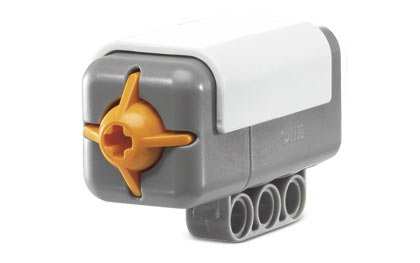
\includegraphics[scale=0.5]{img/sensPress.jpg}
	\caption{Il sensore di pressione}
  \end{center}
\end{figure}\\
Il costruttore della classe \texttt{TouchSensor} permette di
istanziare un nuovo oggetto di tipo \texttt{TouchSensor} connesso
ad una porta del brick NXT.
\begin{lstlisting}
	TouchSensor(ADSensorPort port)
\end{lstlisting}
Dove il parametro \texttt{port} � un'implementazione dell'interfaccia
\texttt{ADSensorPort}, ad esempio \texttt{SensorPort}, che indica
a quale porta � connesso il sensore.\\
\\
La classe \texttt{TouchSensor} mette a disposizione un solo metodo:
\begin{lstlisting}
	/** restituisce vero quando il pulsante � premuto */
	boolean isPressed();
\end{lstlisting} 


\subsection{Il sensore di colore}
Il sensore di colore non � fornito nella normale dotazione di
\emph{Lego}\textregistered~NXT ma deve essere acquistato 
separatamente.\\
Per la gestione di questo sensore, \emph{Lejos} fornisce 
la classe \texttt{ColorSensor}.\\
\begin{figure}
  \begin{center}
	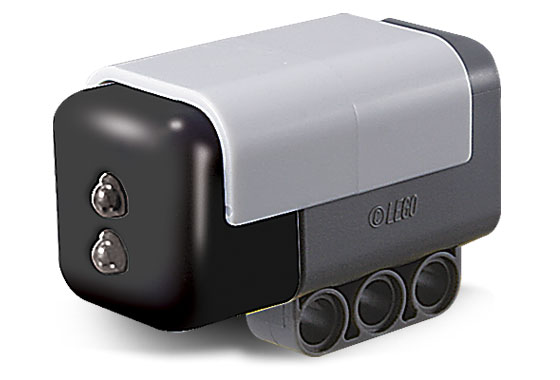
\includegraphics[scale=0.3]{img/sensColor.jpg}
	\caption{Il sensore di colore}
  \end{center}
\end{figure}\\
Il costruttore della classe \texttt{ColorSensor}
\begin{lstlisting}
 ColorSensor(I2CPort port)
\end{lstlisting}
ha come parametro un'implementazione dell'interfaccia
\texttt{I2CPort}, ad esempio \texttt{SensorPort}, che
indichi a quale porta del brick NXT il sensore � connesso.\\
\\
La classe \texttt{ColorSensor} fornisce  seguenti metodi:
\begin{lstlisting}
 /** restituisce la saturazione del blu (0-255)*/
 int getBlue();
 /** restituisce un numero a 0 e 17 che indica il colore letto,
	 0 = nero
	 1 = violetto
	 2 = viola
	 3 = blu
	 4 = verde
	 5 = lime
	 6 = giallo
	 7 = arancione
	 8 = rosso
	 9 = cremisi
	 10 = magenta
	 11 to 16 = pastelli
	 17 = bianco	
	 */	
 int getColorNumber();
 /** restituisce la saturazione del verde (0-255)*/
 int getGreen();
 /** restituisce la saturazione del rosso (0-255)*/
 int getRed(); 
 /** comandi per la calibrazione, si rimanda alla documentazione
	 per maggiori dettagli */
 int initBlackLevel();
 int initWhiteBalance();  
\end{lstlisting}

